
\subsection{Models details}

We used the many-to-one architecture like the one below for our 
classifier.
\begin{figure}[ht]
\vskip 0.2in
\begin{center}
\centerline{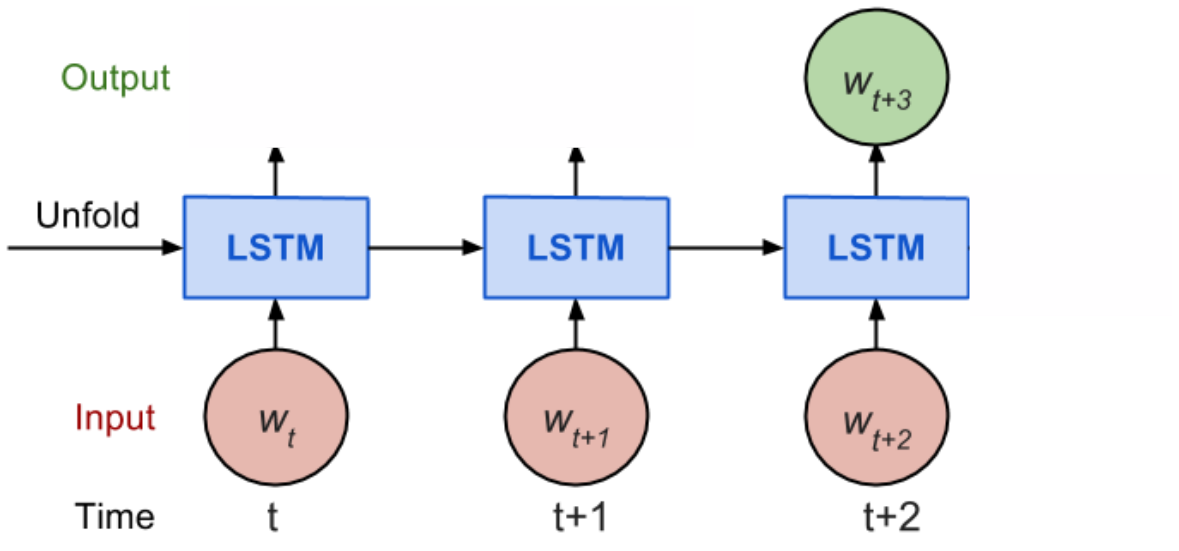
\includegraphics[width=\columnwidth]{manytoone}}
\caption{Many-to-one architecture}
\end{center}
\vskip -0.2in
\end{figure}
We used the last output of the LSTM as our input for the classifier, 
disregarding all the other outputs. The last hidden state contains 
information about about all the sequence through the memory cell. 

\subsection{Results}

\begin{figure}[ht]
\vskip 0.2in
\begin{center}
\centerline{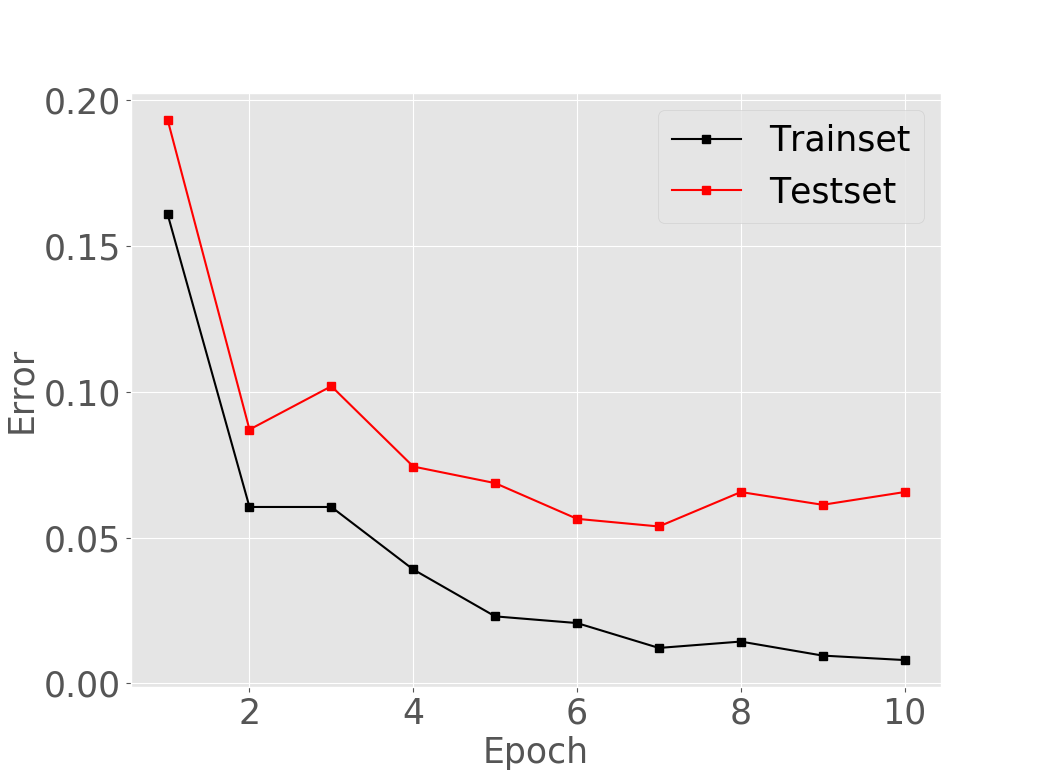
\includegraphics[width=\columnwidth]{gejaclass}}
\caption{Classification error for Austen and Eliot datasets.}
\end{center}
\vskip -0.2in
\end{figure}

\begin{figure}[ht]
\vskip 0.2in
\begin{center}
\centerline{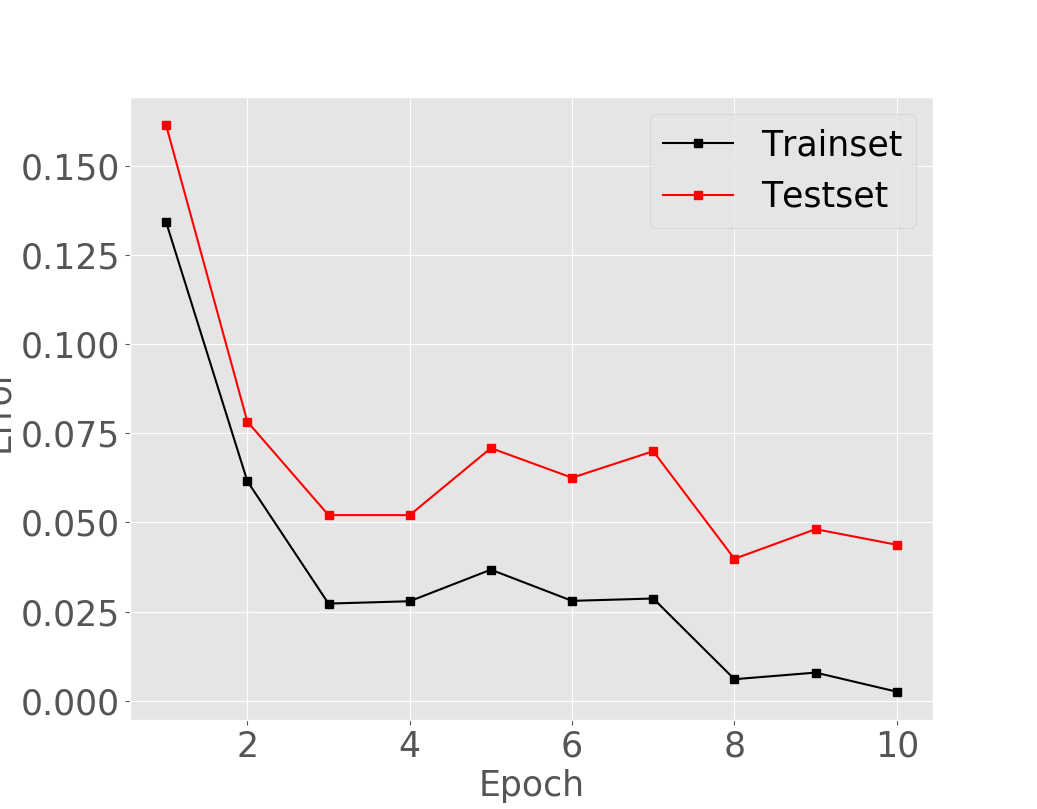
\includegraphics[width=\columnwidth]{gejaclasswithout}}
\caption{Classification error for Austen and Eliot with generic character names}
\end{center}
\vskip -0.2in
\end{figure}
\begin{figure}[ht]
\vskip 0.2in
\begin{center}
\centerline{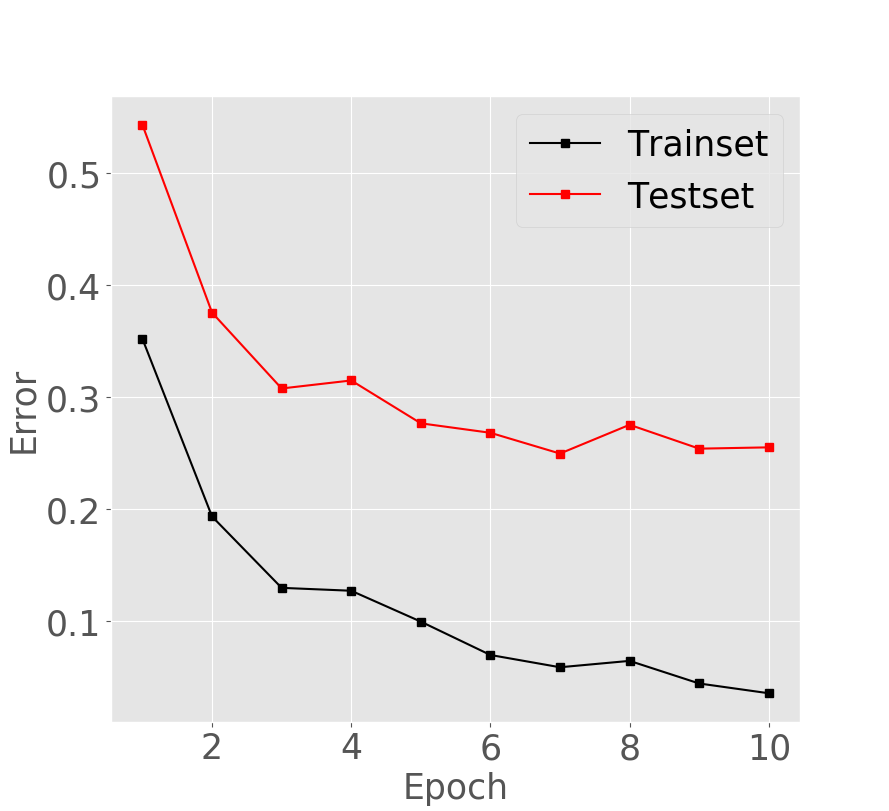
\includegraphics[width=\columnwidth]{yeet}}
\caption{Classification eror for novels from Austen, Eliot, Bronte, Gaskell, Dickens}
\label{fig2}
\end{center}
\vskip -0.2in
\end{figure}
The error we used here is the cross-entropy loss, which is standard for 
classification tasks. We see on our training curves (figure 2) that we 
have reach 96\% for the classification accuracy.

For the text generation models, we used a many-to-many achitecture like 
the one showed in the RNN section with one layer for computational reasons.
LSTMs are with a cell state of 512 dimensions. We trained trough minimization 
of the cross-entropy loss, which is equivalent to \textit{perplexity}; the 
standard metric for language modeling \cite{gravesGenerating}.

\begin{figure}[htbp!]
\begin{tabular}{|l|l|c|}
\hline
Dataset & BPC & Perplexity \\
\hline
Jane Austen & 1.00 & 33 \\
George Eliot& 1.11 & 47 \\
Jane Austen generic names & 1.29  & 88 \\
George Eliot generic names & 1.09 & 43\\
Harry Potter & 1.00 & 33 \\
LOTR & 1.02 & 35 \\
Random quotes & 1.10 & 45 \\
Shakespeare & 0.94 & 26\\
\hline
\end{tabular}
\end{figure}

Examples of generated quotes:
\begin{itemize}\compresslist
    \item `` well , we ' ll do it with a wand , '' said hermione . `` really ?
      '' said harry , looking at each other .
    \item  what looked about this
      way , the black citadel , was far from the
          darkness , the ring was heard , but the sea big was big , and a great
          ring was in his battle .
    \item failure is a beginning of love and a family which comes from god .
    \item  '' that now my mind shall screens his music , '' '' and i to give
      thee my vulgar heaven , '' '' i am your brother .
    \item why i gone that sort man , because he came : they had been oldest to
        look ; i shall be ready to that their clerk , and zebedee 's lay 's long wanted
\end{itemize}
